\documentclass{pizzablatt}

%\geometry{tmargin=1.5cm,bmargin=1.0cm,lmargin=2.60cm,rmargin=2.60cm}

%\setlength{\aufgabenskip}{1.0em}

\begin{document}

\maketitle{2}{Pizzaseminar zur Knotentheorie}{18. September 2013}

\setlength{\unitlength}{1cm}
\begin{picture}(0,0)
  \put(14,-3.5){\vbox{%
    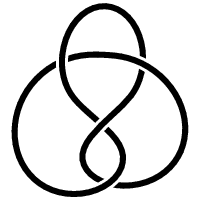
\includegraphics[scale=0.35]{Figure8knot} \\
    \hspace*{1.3em}\tiny Achterknoten
  }}
\end{picture}

\begin{aufgabe}{Kauffman-Klammer und Jones-Polynom in einem konkreten Beispiel}
Berechne Kauffman-Klammer und Jones-Polynom des
Achterknotens.
\end{aufgabe}

\begin{aufgabe}{Kauffman-Klammer und Jones-Polynom unter Spiegelung}
Beweise die Identitäten
\[
 \langle \bar D\rangle = \overline{\langle D\rangle} \qquad \text{und} \qquad V(\bar D)= \overline{V(D)}.
\]
Hierbei ist $D$ ein Diagramm (eine reguläre Projektion eines Knotens oder einer
Verschlingung auf $\RR^2$) und $\bar D$ das an einer Achse des $\RR^2$
gespiegelte Diagramm. Außerdem beizeichnet $\overline P$ das Laurant-Polynom,
das aus $P\in \ZZ[A,A^{-1}]$ durch Vertauschen von $A$ und $A^{-1}$ entsteht.

\emph{Hinweis:} Definiere das Polynom $\overline{\langle\cdot\rangle}$ durch
Regeln analog zur Kauffman-Klammer.
\end{aufgabe}

\begin{aufgabe}{Reidemeister-Bewegungen}
Die Bilder zeigen die Ränder der Seifert-Flächen des
Kleeblattknotens. Benutze die Reidemeister-Bewegungen, um zu zeigen, dass es
tatsächlich Kleeblattknoten sind.

\begin{center}
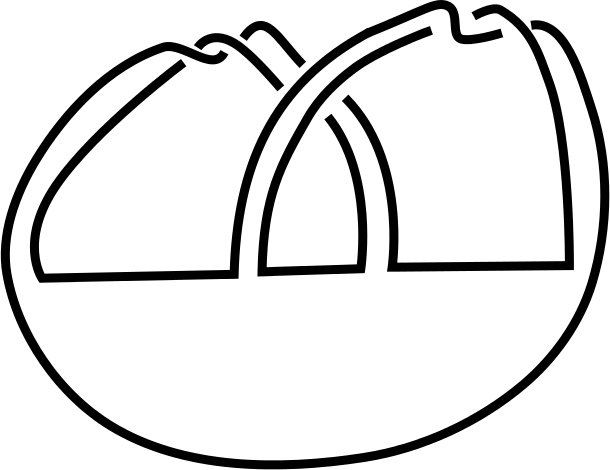
\includegraphics[height=94px]{Kleeblatt1}
\hspace{3em}
\includegraphics[height=94px]{Kleeblatt2}
\end{center}
\end{aufgabe}

\begin{aufgabe}{Seifert-Flächen beliebig hohen Geschlechts}
Sei $K$ ein Knoten mit einer Seifert-Fläche des Geschlechts $g$. Zeige, dass
$K$ auch eine Seifert-Fläche des Geschlechts $g+1$ hat.
\end{aufgabe}

\begin{aufgabe}{Knoten vom Geschlecht Null}
Zeige, dass jeder Knoten mit Geschlecht Null (das heißt, dass es eine in $\RR^3$
eingebettete Kreisscheibe gibt, deren Rand der Knoten ist) äquivalent zum Unknoten
ist. 

\emph{Hinweis:} Approximiere den Knoten durch Polygonzüge und verändere ihn
dann innerhalb der Scheibe.
\end{aufgabe}

\end{document}
